%======================
% Chapter 3 : Related Theory
%======================

\chapter{\scshape Related Theory}

\section{Hardware Description}

\subsection{ESP32 DevKit V1}

The ESP32 DevKit V1 (Espressif Systems) is a dual-core Xtensa LX6 microcontroller operating at up to 240\,MHz, with 520\,KB SRAM, 4\,MB flash, and integrated 802.11\,b/g/n WiFi and Bluetooth 4.2. For SPARK, only the WiFi subsystem is used; Bluetooth is disabled to conserve power. The ESP32 executes both the sensor acquisition ISR at 100\,Hz and the two-layer fall detection pipeline including TFLite Micro CNN inference within the available SRAM and flash envelope. INT8 quantization reduces the 1D CNN model footprint to approximately 80--120\,KB of flash, leaving sufficient headroom for the Arduino~SDK, WiFi stack, and ring-buffer firmware.

\begin{figure}[H]
	\centering
	
\includegraphics[width=0.32\textwidth]{esp32_devkit.png}
	\caption{ESP32 DevKit V1}
	\label{fig:esp32_devkit}
\end{figure}

\subsection{MPU6050 6-Axis IMU}

The InvenSense MPU-6050 integrates a 3-axis MEMS accelerometer ($\pm$2/$\pm$4/$\pm$8/$\pm$16\,g selectable) and a 3-axis MEMS gyroscope ($\pm$250/$\pm$500/$\pm$1000/$\pm$2000$^\circ$/s selectable) on a single die, communicating over I$^2$C at up to 400\,kHz. For SPARK, the accelerometer is configured at $\pm$8\,g full-scale (captures the free-fall and impact spike of a genuine fall without clipping) and the gyroscope at $\pm$500$^\circ$/s. The built-in Digital Motion Processor (DMP) is bypassed in favour of raw register reads at 100\,Hz, enabling direct integration with the complementary filter and sliding window buffer.

\begin{figure}[H]
	\centering
	
\includegraphics[width=0.28\textwidth]{mpu6050.png}
	\caption{MPU6050 6-Axis IMU}
	\label{fig:mpu6050}
\end{figure}

\subsection{Raspberry Pi 4B Gateway}

The Raspberry Pi 4B (4\,GB) serves as the SPARK gateway. It runs the Mosquitto MQTT broker, the FastAPI/Uvicorn backend, PostgreSQL~14 event log, Streamlit dashboard, python-telegram-bot alert service, and the SHAP attribution pipeline. The 4\,GB RAM variant is the target for this project; KEC has one such unit, with a dedicated purchase as contingency if it cannot be allocated. The RPi 4B is powered by a standard 5\,V/3\,A USB-C supply and can operate continuously from AC mains in a care facility or household setting. During development and demonstration, a laptop (minimum 4\,GB RAM, dual-core CPU, Python~3.9+) can substitute as the gateway without code changes.

\begin{figure}[H]
	\centering
	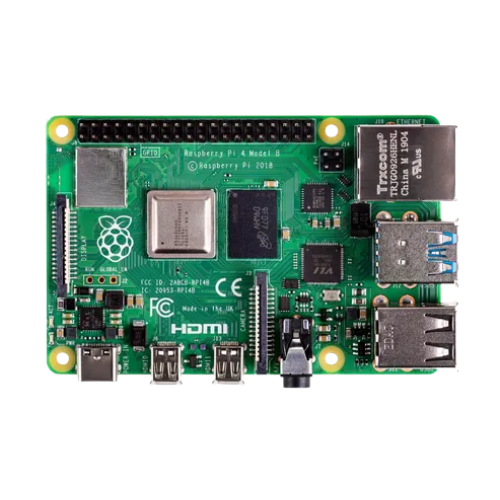
\includegraphics[width=0.32\textwidth]{rpi4b.png}
	\caption{Raspberry Pi 4B Gateway}
	\label{fig:rpi4b}
\end{figure}

\subsection{Power System (Wearable Node)}

The wearable node is powered by a single 18650 lithium-ion cell (2000--3000\,mAh typical) managed by a TP4056 charge controller module (USB-C input, 1\,A charge current). An AMS1117-3.3 low-dropout linear regulator steps the cell voltage (3.0--4.2\,V) to a stable 3.3\,V rail for the ESP32 and MPU6050. An INA219 current/voltage sensor on the power rail provides real-time power telemetry logged to the gateway for battery life characterization. At approximately 80\,mA active current draw, a 2000\,mAh cell provides approximately 25 hours of continuous monitoring.
\subsubsection{18650 Li-ion Cell}

A single 3.7\,V nominal protected lithium-ion battery (typically 2000--3000\,mAh) that serves as the main power source for the wearable node. At an active current draw of approximately 80\,mA, it provides around 25 hours of continuous, uninterrupted fall monitoring.

\begin{figure}[H]
	\centering
	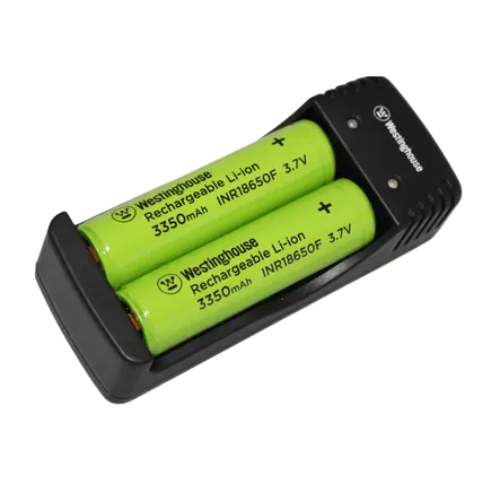
\includegraphics[height=2.6cm,keepaspectratio]{cell_18650.png}
	\caption{18650 Li-ion Cell}
	\label{fig:pwr_cell}
\end{figure}

\subsubsection{TP4056 Charger Module}

A single-cell constant-current/constant-voltage (CC/CV) linear charge controller module with USB-C input. It regulates a 1\,A charging current to safely recharge the 18650 cell and provides safety cutoffs (overcharge protection at 4.2\,V and over-discharge protection at 2.5\,V).

\begin{figure}[H]
	\centering
	
\includegraphics[height=2.6cm,keepaspectratio]{tp4056.png}
	\caption{TP4056 Charger Module}
	\label{fig:pwr_tp4056}
\end{figure}

\subsubsection{AMS1117-3.3}

A low-dropout (LDO) linear voltage regulator that steps down the varying voltage of the 18650 cell (3.0\,V to 4.2\,V) to a fixed, stable 3.3\,V power rail. This stable voltage is required to safely power the ESP32 microcontroller and the MPU6050 IMU sensor.

\begin{figure}[H]
	\centering
	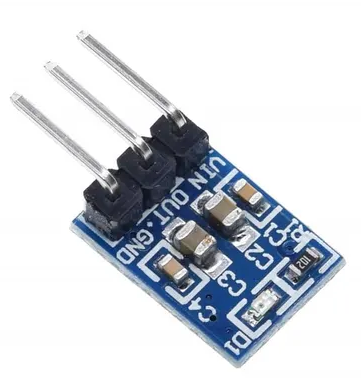
\includegraphics[height=2.6cm,keepaspectratio]{ams1117.png}
	\caption{AMS1117-3.3 LDO}
	\label{fig:pwr_ldo}
\end{figure}

\subsubsection{INA219 Sensor}

A bi-directional current and voltage monitor module connected over I2C to the power rail. It provides real-time power telemetry, logging current draw and voltage levels to the gateway to help characterize battery life during continuous operation.

\begin{figure}[H]
	\centering
	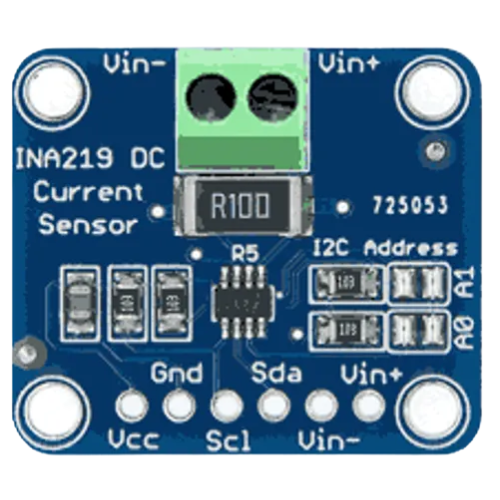
\includegraphics[height=2.6cm,keepaspectratio,trim=0 0 7bp 0,clip]{ina219.png}
	\caption{INA219 Sensor}
	\label{fig:pwr_ina219}
\end{figure}

\subsection{Mechanical Mounting and Support Components}

Beyond the core compute, sensing, and power modules, the wearable node relies on a set of mechanical mounting and low-level support components for physical attachment and circuit integration.

\subsubsection{Velcro Wrist/Chest Strap}

An adjustable Velcro strap used to secure the wearable enclosure to the wrist or chest of the user, allowing the accelerometer and gyroscope to reliably capture body motion during a fall event.

\begin{figure}[H]
	\centering
	
\includegraphics[height=2.6cm,keepaspectratio]{velcro_strap.png}
	\caption{Velcro Wrist/Chest Strap}
	\label{fig:velcro_strap}
\end{figure}

\subsubsection{Chest Strap Mount}

An elasticated chest-mount harness offering an alternative attachment point to the wrist strap, used during controlled fall data collection to evaluate sensor placement sensitivity on detection accuracy.

\begin{figure}[H]
	\centering
	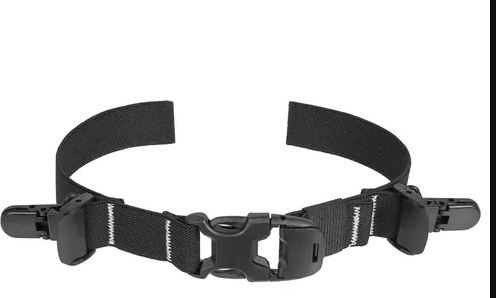
\includegraphics[height=2.6cm,keepaspectratio]{chest_strap.png}
	\caption{Chest Strap Mount}
	\label{fig:chest_strap}
\end{figure}

\subsubsection{USB-C Cables}

Standard USB-C cables used to power and program the ESP32 DevKit V1 boards and to charge the TP4056 module during bench testing.

\begin{figure}[H]
	\centering
	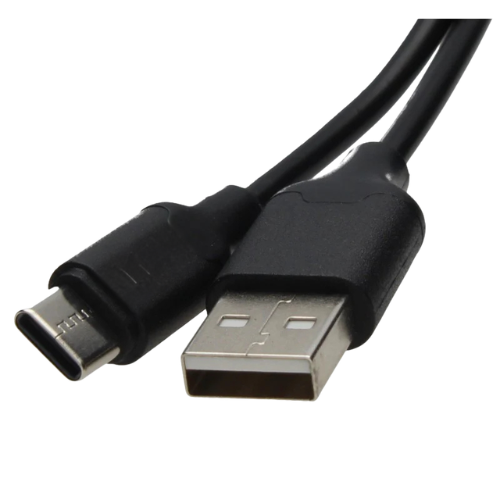
\includegraphics[height=2.6cm,keepaspectratio]{micro_usb_cable.png}
	\caption{USB-C Cable}
	\label{fig:micro_usb_cable}
\end{figure}

\subsubsection{MicroSD Card}

A 32\,GB MicroSD card used as the boot and storage medium for the Raspberry Pi 4B gateway, hosting the operating system, PostgreSQL event log, and locally cached SHAP attribution outputs.

\begin{figure}[H]
	\centering
	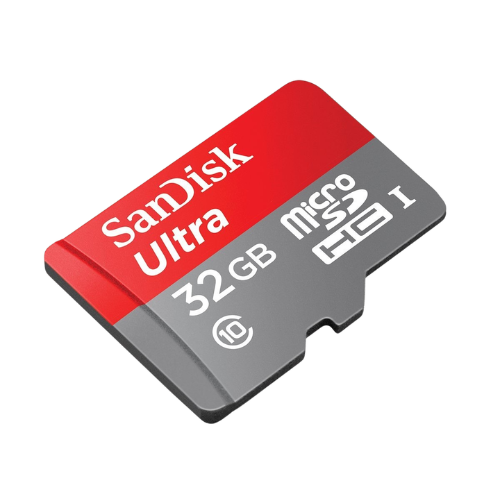
\includegraphics[height=2.6cm,keepaspectratio]{microsd.png}
	\caption{MicroSD Card (32\,GB)}
	\label{fig:microsd}
\end{figure}

\subsubsection{Passive Components}

Assorted resistors and capacitors used on the wearable node breadboard for signal conditioning, decoupling, and pull-up/pull-down configuration around the ESP32, INA219, and AMS1117 circuitry.

\begin{figure}[H]
	\centering
	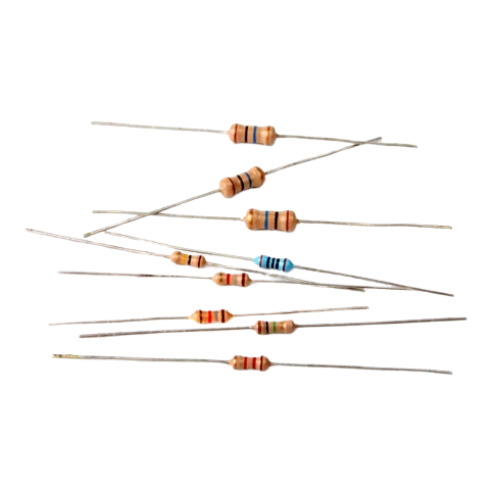
\includegraphics[height=2.6cm,keepaspectratio]{resistor.png}
	\caption{Resistor}
	\label{fig:resistor}
\end{figure}

\begin{figure}[H]
	\centering
	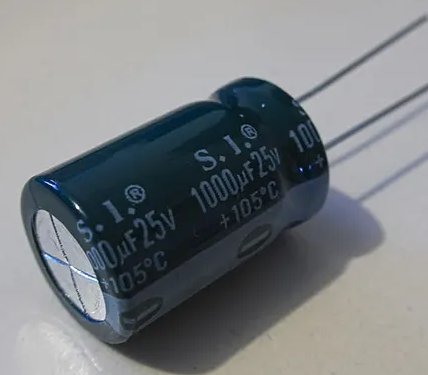
\includegraphics[height=2.6cm,keepaspectratio]{capacitor.png}
	\caption{Capacitor}
	\label{fig:capacitor}
\end{figure}

\section{Software Description}

\subsection{Two-Layer Detection Architecture}

The detection pipeline implements a gated dual-layer structure. Layer~1 is a deterministic threshold pre-filter executed in the ESP32 ISR at 100\,Hz. It computes the resultant acceleration magnitude $|a| = \sqrt{a_x^2 + a_y^2 + a_z^2}$ and the angular velocity magnitude $|\omega| = \sqrt{\omega_x^2 + \omega_y^2 + \omega_z^2}$. A \texttt{PRE\_FALL} flag is raised when $|a|$ exceeds 2.5\,g (free-fall proxy spike) followed by $|a| < 0.5$\,g for more than 300\,ms (post-impact rest phase). This threshold logic mirrors the deterministic safety logic of ISO~13482:2014 (safety requirements for personal care robots). Layer~1 latency is below 5\,ms and incurs no inference cost.

When \texttt{PRE\_FALL} is raised, Layer~2 is invoked: a 2-second sliding window of $(a_x, a_y, a_z, \omega_x, \omega_y, \omega_z)$ at 100\,Hz is assembled (200 samples $\times$ 6 channels $=$ 1200 INT8 values), normalized using StandardScaler parameters baked into the firmware at training time, and fed to the TFLite Micro 1D CNN. The CNN produces a fall probability score $P(\text{FALL}) \in [0, 1]$. If $P(\text{FALL}) > 0.85$, a \texttt{CONFIRMED\_FALL} event is serialized as a JSON payload and transmitted to the gateway over WiFi via MQTT.

\subsection{1D CNN Architecture}

The 1D CNN consists of: Conv1D(32 filters, kernel 5) $\rightarrow$ ReLU $\rightarrow$ MaxPool1D(2) $\rightarrow$ Conv1D(64 filters, kernel 3) $\rightarrow$ ReLU $\rightarrow$ GlobalAveragePooling1D $\rightarrow$ Dense(32, ReLU) $\rightarrow$ Dense(2, Softmax). The model is trained in TensorFlow/Keras on UCI MHEALTH \cite{banos2014mhealthdroid} and SisFall \cite{sucerquia2017sisfall} datasets with self-collected Nepal-context data as a fine-tuning set. INT8 post-training quantization via the TFLite Converter produces a C array for inclusion in the PlatformIO build.

\subsection{SHAP Explainability Pipeline}

SHAP (SHapley Additive exPlanations) \cite{lundberg2017shap} assigns to each input feature $i$ an attribution value $\phi_i$ satisfying local accuracy ($f(x) = \phi_0 + \sum_i \phi_i$), missingness, and consistency axioms. For each \texttt{CONFIRMED\_FALL} event, the gateway computes SHAP values for the six IMU channel features (peak values of $a_x, a_y, a_z, \omega_x, \omega_y, \omega_z$ extracted from the 2-second window) using the \texttt{shap} Python library's TreeExplainer or KernelExplainer on the trained CNN output. The top contributing feature (e.g., \texttt{az\_peak} with 42\% of fall confidence) and the full SHAP vector are stored in the PostgreSQL \texttt{fall\_events} table and displayed on the Streamlit dashboard alongside the fall event log. This provides care staff with an auditable rationale for every alert --- a capability absent from all commercial and published academic fall detection systems.

\subsection{Gateway Software Architecture}

The gateway implements three software design patterns documented in the thesis Chapter~3 (OOSE alignment):

\textbf{Factory Pattern} decouples the detection node abstraction from its concrete implementations. A \texttt{FallDetector} abstract base class handles WiFi transmission, event serialization, and power management; \texttt{ThresholdDetector} (Layer~1) and \texttt{CNNDetector} (Layer~2) are concrete subclasses.

\textbf{Observer Pattern} implements the alert ecosystem. The FastAPI gateway is the Subject; Streamlit dashboard, Telegram bot, PostgreSQL logger, and PDF report generator are Observers subscribed to \texttt{CONFIRMED\_FALL} events. Adding a new alert channel (e.g., SMS) requires adding a new Observer without modifying the gateway core.

\textbf{Strategy Pattern} implements the configurable sensitivity profiles. A \texttt{FallDetectionStrategy} interface is implemented by three concrete strategies: \texttt{HighSensitivity} (elderly, bed-ridden), \texttt{Standard} (default), and \texttt{SportMode} (active ADL). Threshold parameters are loaded from the user profile at gateway startup; no firmware reflash is required to switch profiles.